\section{The control loop}
\subsection{}

\begin{frame}
\frametitleTC{The control loop and its actors}
\framesubtitleTC{}
\myPause
 \begin{itemize}[<+-| alert@+>]
 \item General representation:
       \begin{center}
        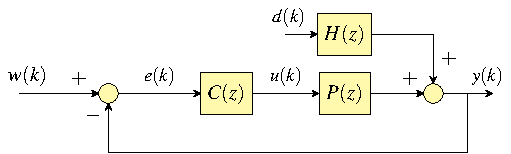
\includegraphics[width=0.50\columnwidth]{./Unit-04/img/ControlLoop.pdf}
       \end{center}
 \item Notation:
       \begin{itemize}[<+-| alert@+>]
       \item $w(k)$ is the \TC{set point} or \TC{reference};
       \item $y(k)$ is the \TC{controlled variable};
       \item $e(k)$ is the \TC{error};
       \item $u(k)$ is the \TC{control signal};
       \item $d(k)$ is a \TC{disturbance};
       \item $P(z)$ and $H(z)$ compose the \TC{controlled system} model;
       \item $C(z)$ is the \TC{controller} transfer function.
       \end{itemize}
 \end{itemize}
\end{frame}

\begin{frame}
\frametitleTC{The control loop and its actors}
\framesubtitleTC{}
 \begin{center}
  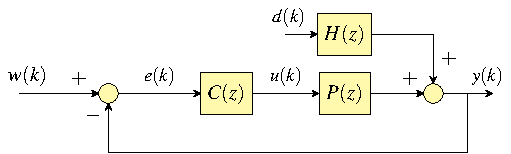
\includegraphics[width=0.40\columnwidth]{./Unit-04/img/ControlLoop.pdf}
 \end{center}
 \begin{itemize}[<+-| alert@+>]
 \item \vspace{-2mm} Some remarks:
       \begin{itemize}[<+-| alert@+>]
       \item we assume that the \TC{measurement} of $y$ reaching the node that generates the error,
             is exact (no disturbance on the feedback line) and instantaneous (no dynamic block
             on that line either);
       \item this may be \emph{very} questionable when some sensor is in the \emph{arena}, thus for\\
             example is not always assumed in process control, robotics and the like;
       \item however in computers most measurements are in fact the measured\\
             quantity itself (e.g., the one timer firing preemption interrupts and\\
             accounting CPU usage);
       \item this is an important simplification to exploit when applying control\\
             to computing system,
       \item with the exception of more ``physical'' controls (temperature, power,...)\\
             where sensor dynamics may be of some concern.
       \end{itemize}
 \end{itemize}
\end{frame}

\begin{frame}
\frametitleTC{Intermezzo}
\framesubtitleTC{Composing blocks in a feedback structure (we still miss this besides series and parallel)}
 \begin{center}
  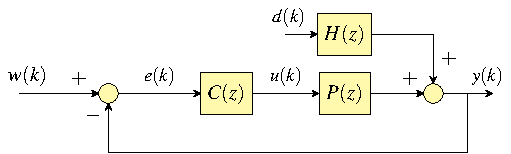
\includegraphics[width=0.40\columnwidth]{./Unit-04/img/ControlLoop.pdf}
 \end{center}\myPause
 \begin{itemize}[<+-| alert@+>]
 \item We need to compute the transfer functions from $w$ and $d$ to $y$ and $u$.
 \item To this end, imagine to cut the loop (for example right of the node summing the outputs of $P$ and $H$).
 \item Equating the left and the right side of this fictitious cut we have
       \begin{displaymath}
        H(z)d(k) + P(z)C(z) \left(w(k)-y(k) \right) = y(k),
       \end{displaymath}
 \item whence rearranging
       \begin{displaymath}
        y(k) = \frac{P(z)C(z)}{1+P(z)C(z)} w(k) + \frac{H(z)}{1+P(z)C(z)} d(k).
       \end{displaymath}
 \end{itemize}
\end{frame}

\begin{frame}
\frametitleTC{Intermezzo}
\framesubtitleTC{Composing blocks in a feedback structure}
\myPause
 \begin{itemize}[<+-| alert@+>]
 \item We adopt from now on the convention of calling $G_{ba}(z)$ the transfer function from $a(k)$ to $b(k)$
       when convenient --- btw, mind the subscript order. 
 \item We also recall the operatorial meaning of a transfer function, and that it represents the \TC{effect}
       of a certain input to a certain output. In other words, in our case we should for completeness write
       \begin{displaymath}
        G_{yw}(z) = \left. \frac{y(k)}{w(k)} \right|_{d(k)=0}, \qquad
        G_{yd}(z) = \left. \frac{y(k)}{d(k)} \right|_{w(k)=0},
       \end{displaymath}
       but we drop part of the notation for simplicity.
 \item Summing up, we have
       \begin{displaymath}
        G_{yw}(z) = \frac{P(z)C(z)}{1+P(z)C(z)}, \qquad
        G_{yd}(z) = \frac{H(z)}{1+P(z)C(z)}.
       \end{displaymath}
 \end{itemize}
\end{frame}

\begin{frame}
\frametitleTC{Intermezzo}
\framesubtitleTC{Composing blocks in a feedback structure}
\myPause
 \begin{center}
  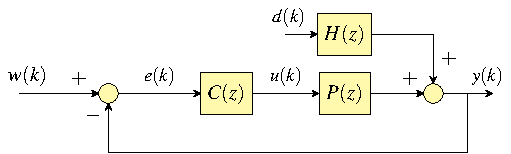
\includegraphics[width=0.40\columnwidth]{./Unit-04/img/ControlLoop.pdf}
 \end{center}\myPause
 \begin{itemize}[<+-| alert@+>]
 \item Reasoning in the same way for the output $u(k)$ -- details left as an exercise -- we have
       \begin{displaymath}
        G_{uw}(z) =  \frac{C(z)}{1+P(z)C(z)}, \qquad
        G_{ud}(z) = -\frac{C(z)H(z)}{1+P(z)C(z)}.
       \end{displaymath}
 \end{itemize}
\end{frame}

\begin{frame}
\frametitleTC{The control loop and its actors}
\framesubtitleTC{Main transfer functions of interest}
\myPause
 \begin{itemize}[<+-| alert@+>]
 \item Loop:
       \begin{displaymath}
        L(z) := P(z)C(z).
       \end{displaymath}
 \item From set point to controlled variable and control signal:
       \begin{displaymath}
        G_{yw}(z) = \frac{L(z)}{1+L(z)}, \qquad
        G_{uw}(z) = \frac{C(z)}{1+L(z)}.
       \end{displaymath}
 \item From disturbance to controlled variable and control signal:
       \begin{displaymath}
        G_{yd}(z) =  \frac{H(z)}{1+L(z)}, \qquad
        G_{ud}(z) = -\frac{C(z)H(z)}{1+L(z)}.
       \end{displaymath}
 \end{itemize}
\end{frame}

\begin{frame}
\frametitleTC{The control part of the loop}
\framesubtitleTC{Functional view}
\myPause
 \begin{itemize}[<+-| alert@+>]
 \item For the loop to operate
       \begin{itemize}[<+-| alert@+>]
       \item an \TC{event generator} triggers a new control action (periodically or on demand,\\
             here we stick to the former case);
       \item a \TC{sensor} is activated to get $y(k)$;
       \item the \TC{controller} $C(z)$ is invoked, and evolves as dynamic system by one step,
             \begin{itemize}[<+-| alert@+>]
             \item updating its state
             \item and then computing the new control $u(k)$;
             \end{itemize}
       \item an \TC{actuator} is activated to act on the process;
       \item and finally the system waits for a new event.
       \end{itemize}
 \item \vfill This view is quite easily related to CS frameworks such as\\
       the MAPE(-K).
 \item However, to design the controller, another view is preferable.
 \end{itemize}
\end{frame}

\begin{frame}
\frametitleTC{The control part of the loop}
\framesubtitleTC{Systemic view}
\myPause
 \begin{itemize}[<+-| alert@+>]
 \item For the loop to operate correctly
       \begin{itemize}[<+-| alert@+>]
       \item the closed-loop system must be asymptotically stable (more detail on this matter coming soon);
       \item the reference-to-output transfer function $G_{yw}(z)$, and/or the disturbance-to-output one $G_{yd}(z)$,
             must yield ``acceptable'' time responses in the presence of \TC{expectable} signals $w(k)$ and $d(k)$;
       \item the controller must be \TC{realisable}, i.e., the order of the numerator of $C(z)$ cannot exceed
             that of the denominator;
       \item in the opposite case, to explain the term ``realisable'', the controller\\
             output would depend on FUTURE samples of its input, which clearly\\ 
             is impossible to realise.
       \item We already saw that the above degree relationship is a structural\\
             property of any properly defined transfer function, incidentally.
       \end{itemize}
 \end{itemize}
\end{frame}

\begin{frame}\mccz
\frametitleTC{Time to start assembling our puzzle}
\framesubtitleTC{}
\myPause
 \begin{columns}
  \column[T]{0.35\textwidth}
   \only<2->{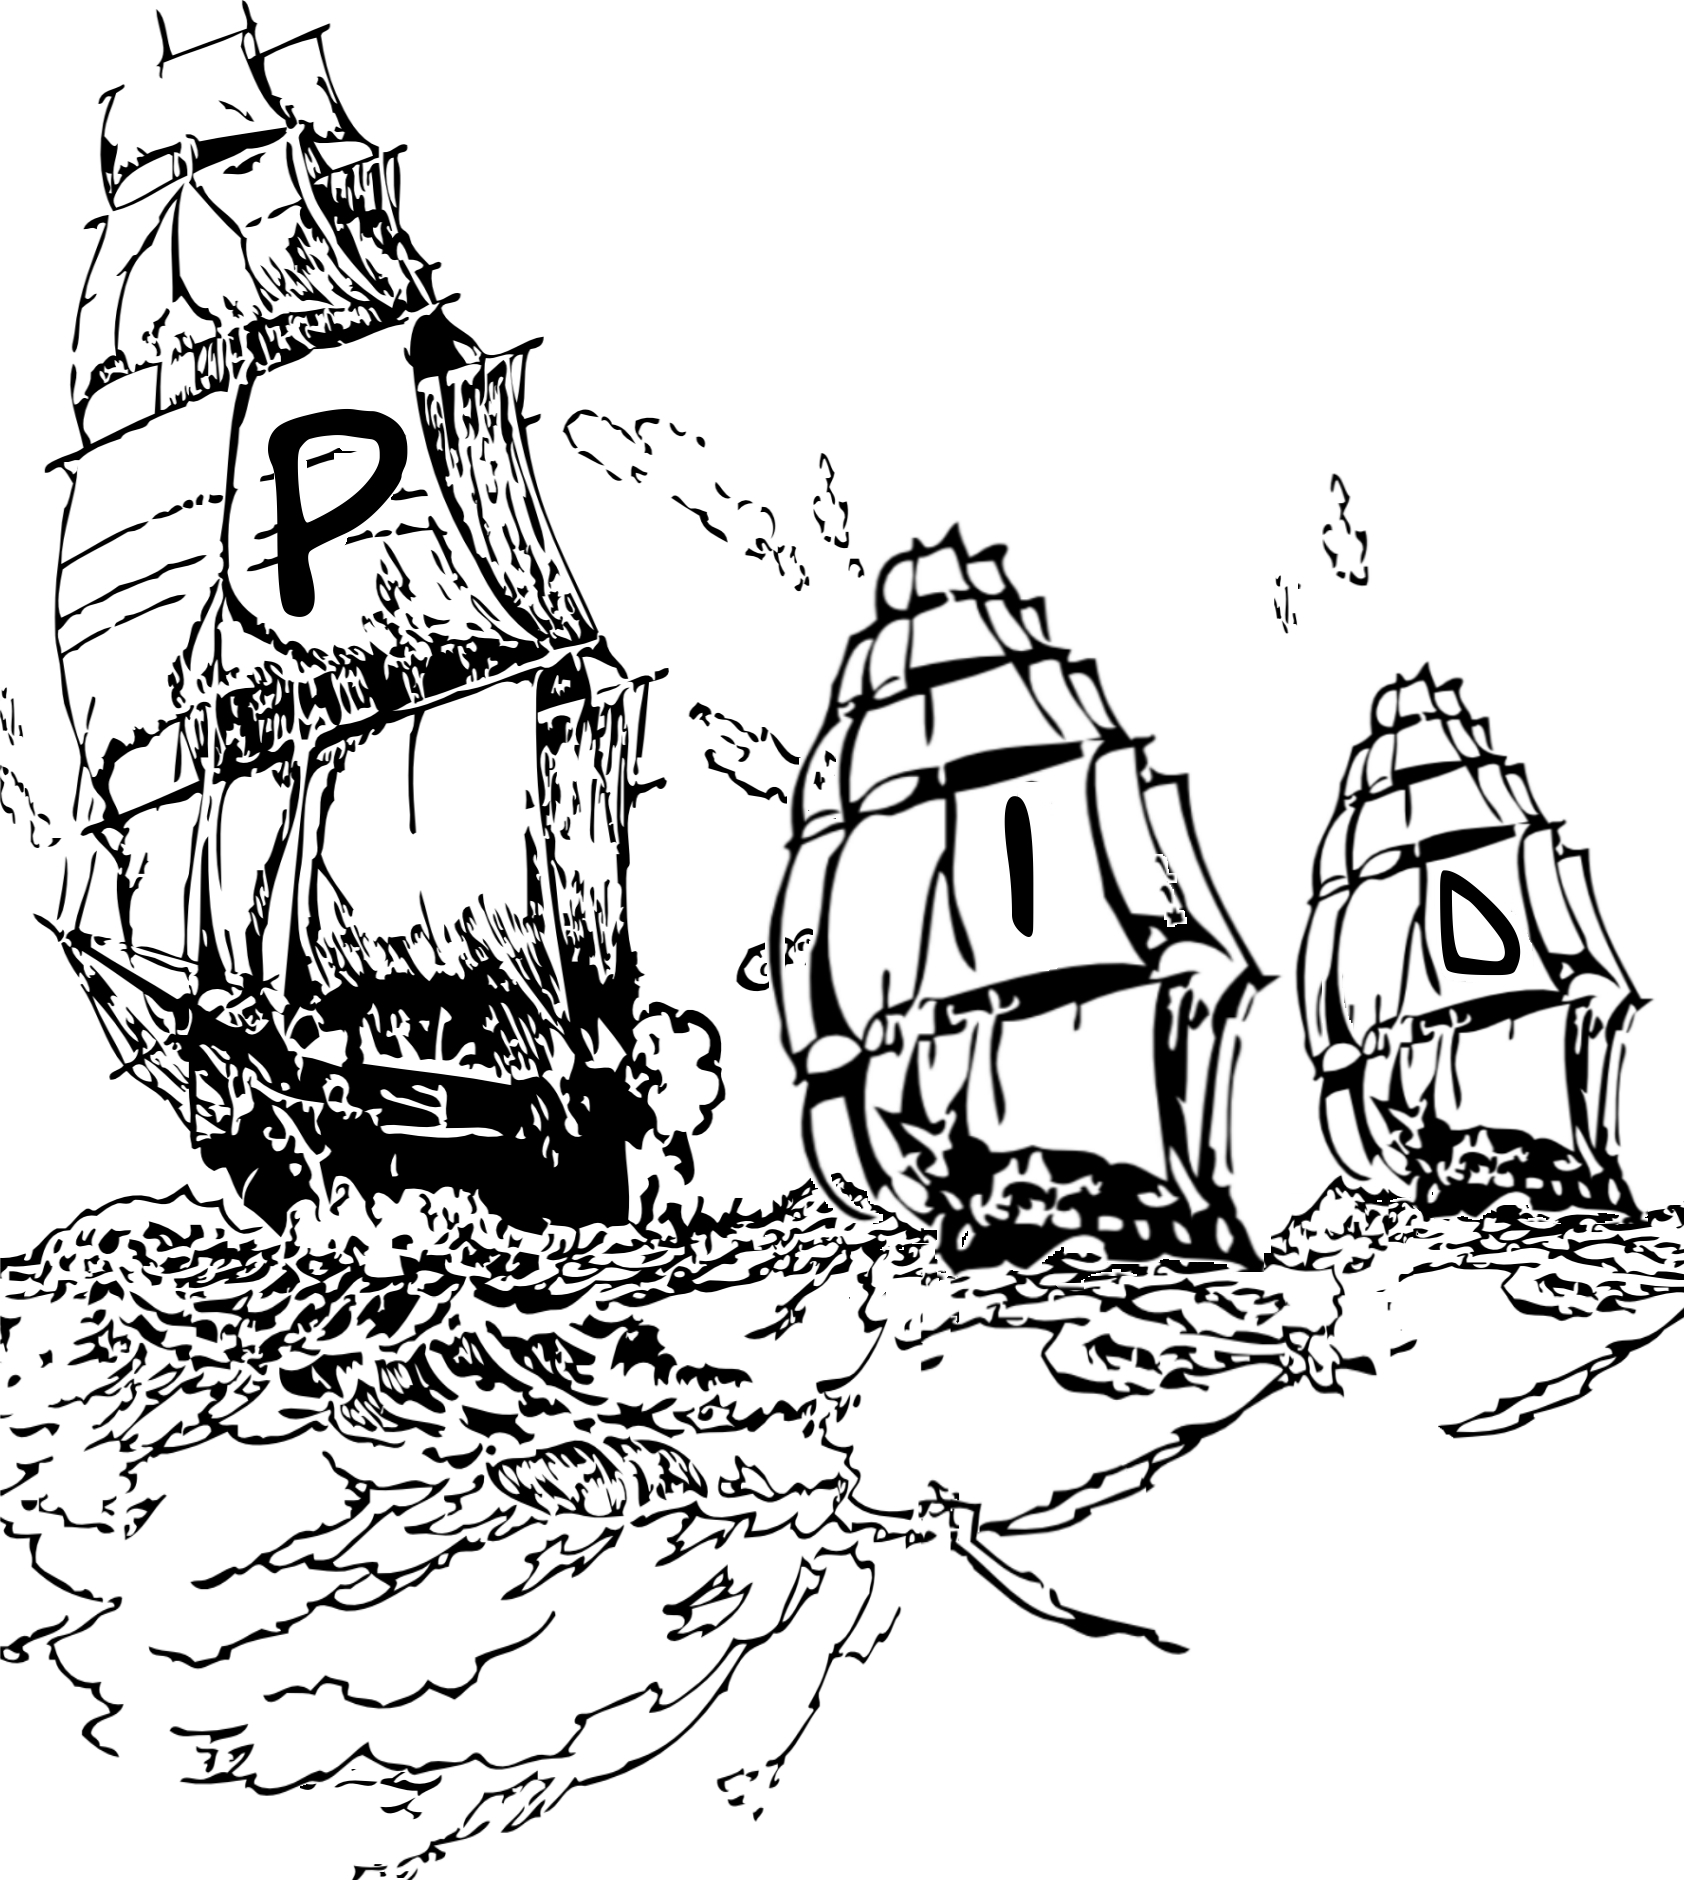
\includegraphics[height=6cm]{./Unit-04/img/PIDsOnTheHorizon_cc0.jpg}}
  \column[T]{0.65\textwidth}
   \begin{itemize}[<+-| alert@+>]
   \item First we shall learn a feedback control synthesis\\
         technique named ``direct'',
   \item then we shall discuss the relationships between\\
         the dynamic structure of the process\\
         and that of the controller,
   \item finally coming, as a quite natural\\
         consequence, to anticipate\\
         the PID control law. 
   \end{itemize}
 \end{columns}
\end{frame}


